\section{Baseline Surrogate Models}
A common approach for constructing data-driven reservoir surrogates is to formulate a mapping from local, cell-wise state inputs at timestep $t$ directly to the absolute cell pressure at the subsequent timestep $t+1$:
\begin{equation}
\label{eq:direct_p}
P_i(t+1) = f(X_{\text{local}, i}(t))
\end{equation}
where $X_{\text{local}, i}(t)$ is a feature vector containing static cell properties, the current state, and dynamic well controls. To evaluate this formulation, we trained and evaluated three baseline models on the native irregular PEBI mesh:
\begin{enumerate}
    \item \textbf{Persistence Baseline}: A parameter-free physical baseline assuming zero state change over the interval, defined by $\hat{P}_i(t+1) = P_i(t)$.
    \item \textbf{Linear Regression (OLS)}: A standard ordinary least-squares regression mapping the cell-local feature vector to the target pressure.
    \item \textbf{Multilayer Perceptron (MLP)}: A fully connected neural network with a $(128, 64)$ hidden architecture, LeakyReLU activations, and trained using the Adam optimizer with a learning rate of $10^{-3}$.
\end{enumerate}

Evaluating these baseline configurations on the independent test set (Case 5) yielded metrics that, at first glance, appear outstanding. As summarized in Table~\ref{tab:baseline_results}, the MLP model achieves an $R^2 = 0.9955$ with an RMSE of 3.42~bar. Similarly, the linear OLS model reaches an $R^2 = 0.9952$ and an RMSE of 3.53~bar. Crucially, the parameter-free Persistence model achieves a high coefficient of determination ($R^2 = 0.9931$) and an RMSE of 4.22~bar, despite having no knowledge of reservoir physics or active well schedules.

\subsection{The Autocorrelation Trap}
The exceptionally high performance metrics of these baseline models represent a deceptive machine learning artifact. Because pressure fields in porous media evolve smoothly over the reporting interval ($\Delta t = 5$~days), the next-step pressure $P(t+1)$ is highly autocorrelated with the current pressure $P(t)$. The Persistence baseline highlights that any regressor learning to output a value close to its input will achieve a near-unity $R^2$ on the absolute pressure target, regardless of its underlying physical correctness. 

Quantitatively, the trained MLP improves upon the parameter-free Persistence model by only $0.80$~bar in RMSE ($3.42$~bar vs. $4.22$~bar)---a marginal gain of 18.9\% that carries no guarantee of physical flow consistency. In the reservoir surrogate literature, direct absolute pressure $R^2$ values are frequently reported without reference to a persistence baseline, which risks inflating the perceived accuracy of the emulator~\cite{pal2021mlhistory}. We therefore recommend that future surrogate evaluations always report performance on the pressure-change target alongside absolute pressure metrics to establish a meaningful skill score. The comparison of baseline model RMSE under both targets is visualized in Fig.~\ref{fig:baseline_comparison}.

\begin{table*}[t]
\centering
\caption{Baseline Model Performance Comparison on Test Set (Case 5)}
\label{tab:baseline_results}
\begin{tabular}{llcccc}
\toprule
\textbf{Target Formulation} & \textbf{Model} & \textbf{RMSE (bar)} & \textbf{MAE (bar)} & \textbf{Relative Error} & \textbf{$R^2$} \\
\midrule
\textbf{Direct Pressure ($P_{t+1}$)} 
 & Persistence & 4.2180 & 2.0068 & 0.0198 & 0.9931 \\
 & Linear Regression & 3.5266 & 1.3307 & 0.0114 & 0.9952 \\
 & MLP (128-64) & 3.4227 & 1.2009 & 0.0119 & 0.9955 \\
\midrule
\textbf{Pressure Change ($\Delta P$)} 
 & Persistence ($\Delta P = 0$) & 4.2180 & 3.5177 & 0.2043 & -0.0198 \\
 & Linear Regression & 4.1756 & 3.4870 & 0.2030 & 0.0007 \\
 & MLP (128-64) & 3.3614 & 2.5611 & 0.1535 & 0.3524 \\
\bottomrule
\end{tabular}
\end{table*}


\begin{figure}[htbp]
    \centering
    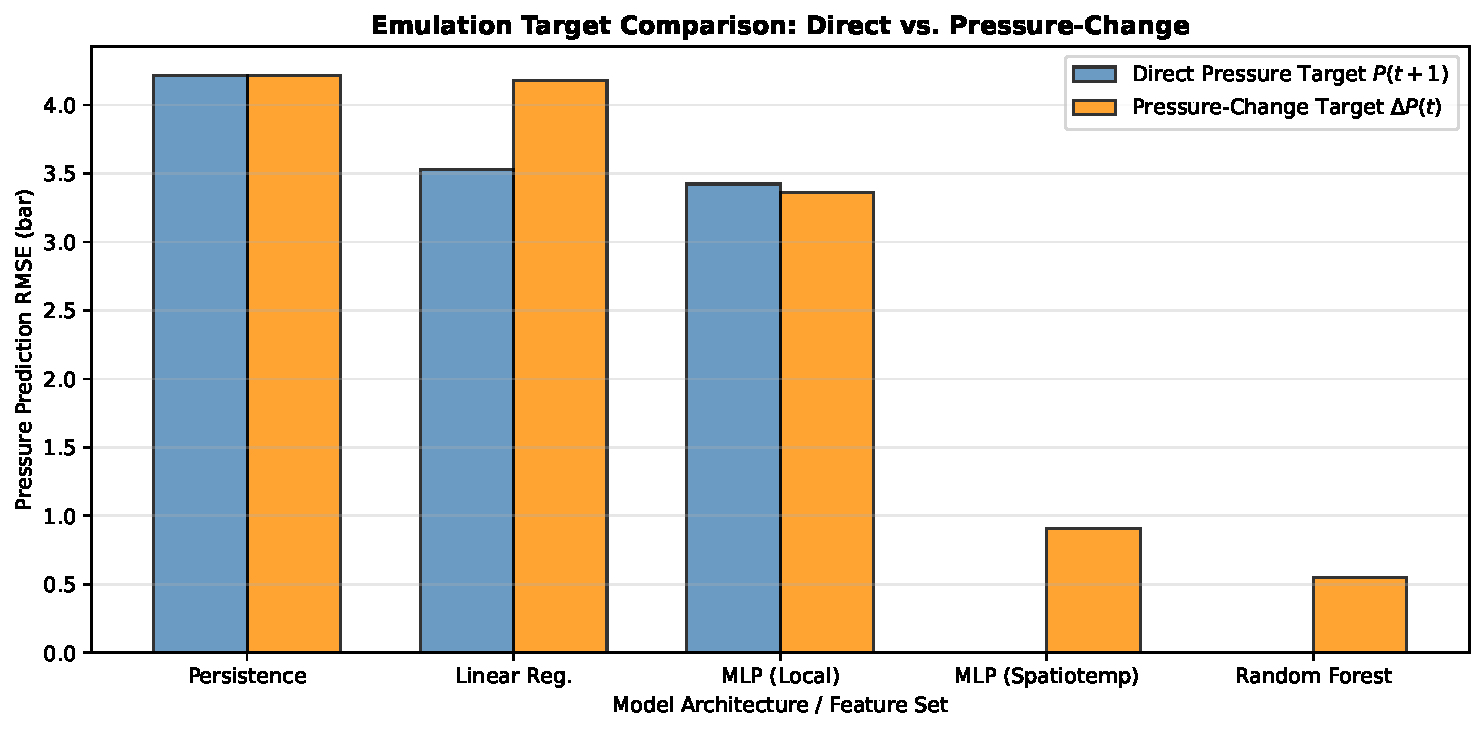
\includegraphics[width=0.95\columnwidth]{figures/fig4_baseline_comparison}
    \caption{Forecasting RMSE (bar) comparison on Test Case 5 for the direct pressure ($P_{t+1}$) versus the pressure-change ($\Delta P$) targets across the three baseline models.}
    \label{fig:baseline_comparison}
\end{figure}
